\fancyfoot[C]{Sandri}
\section{Hauptplatine(Athena Control Hub)}
	Die Hauptplatine soll ein Shield(Aufsteckplatine) f�r den Boardcomputer sein. Auf dem Shield sollen alle Komponenten des Autos angeschlossen werden k�nnen. Die Platine besteht aus folgenden Komponenten:
	
		\begin{itemize}
			
			\item Stecker f�r Spannungswandler liefert 12V und 5V an die Platine
			
			\item ESP32 Mikrocontroller zum Einlesen und Senden aller Sensordaten an den Boardcomputer, weiters kontrolliert er die LED-Beleuchtung
			
			\item Stecker f�r 6 Temperaturtsensoren, welche im Auto verteilt sind
			
			\item Stecker f�r 4 12V PWM-L�fter, welche vom ESP32 geregelt werden k�nnen
			
			\item Stecker f�r die OctoSonar-Platine, welche bis zu 16Ultraschallsensoren einlesen kann
			
			\item Stecker f�r beide IMUs(linearer Beschleunigungssensor, Gyroskop und Magnetometer)
			
			\item Stecker f�r den Einschalter
			
			\item Stecker f�r die Antisparkswitch
			
			\item Stecker um Versorgungsspannung zu messen
			
			\item Stecker f�r vordere und hinter LED-Beleuchtung
			
			\item Stecker die unbelegte Ausg�nge von Optkopplern f�r zuk�nftige Erweiterung hinausf�hren
			
			\item RGB-Status LEDs die den aktuellen Status jeder Komponente darstellen k�nnen
			
			\item Sensor- und Kontrolllogikschaltungen
			
		\end{itemize}
		
		In der Mitte der Platine ist des weiteren ein Loch um dem L�fter vom Boardcomputer ausreichend K�hlleistung zu gew�hrleisten.
		
		\begin{figure}[H]
			\centering
			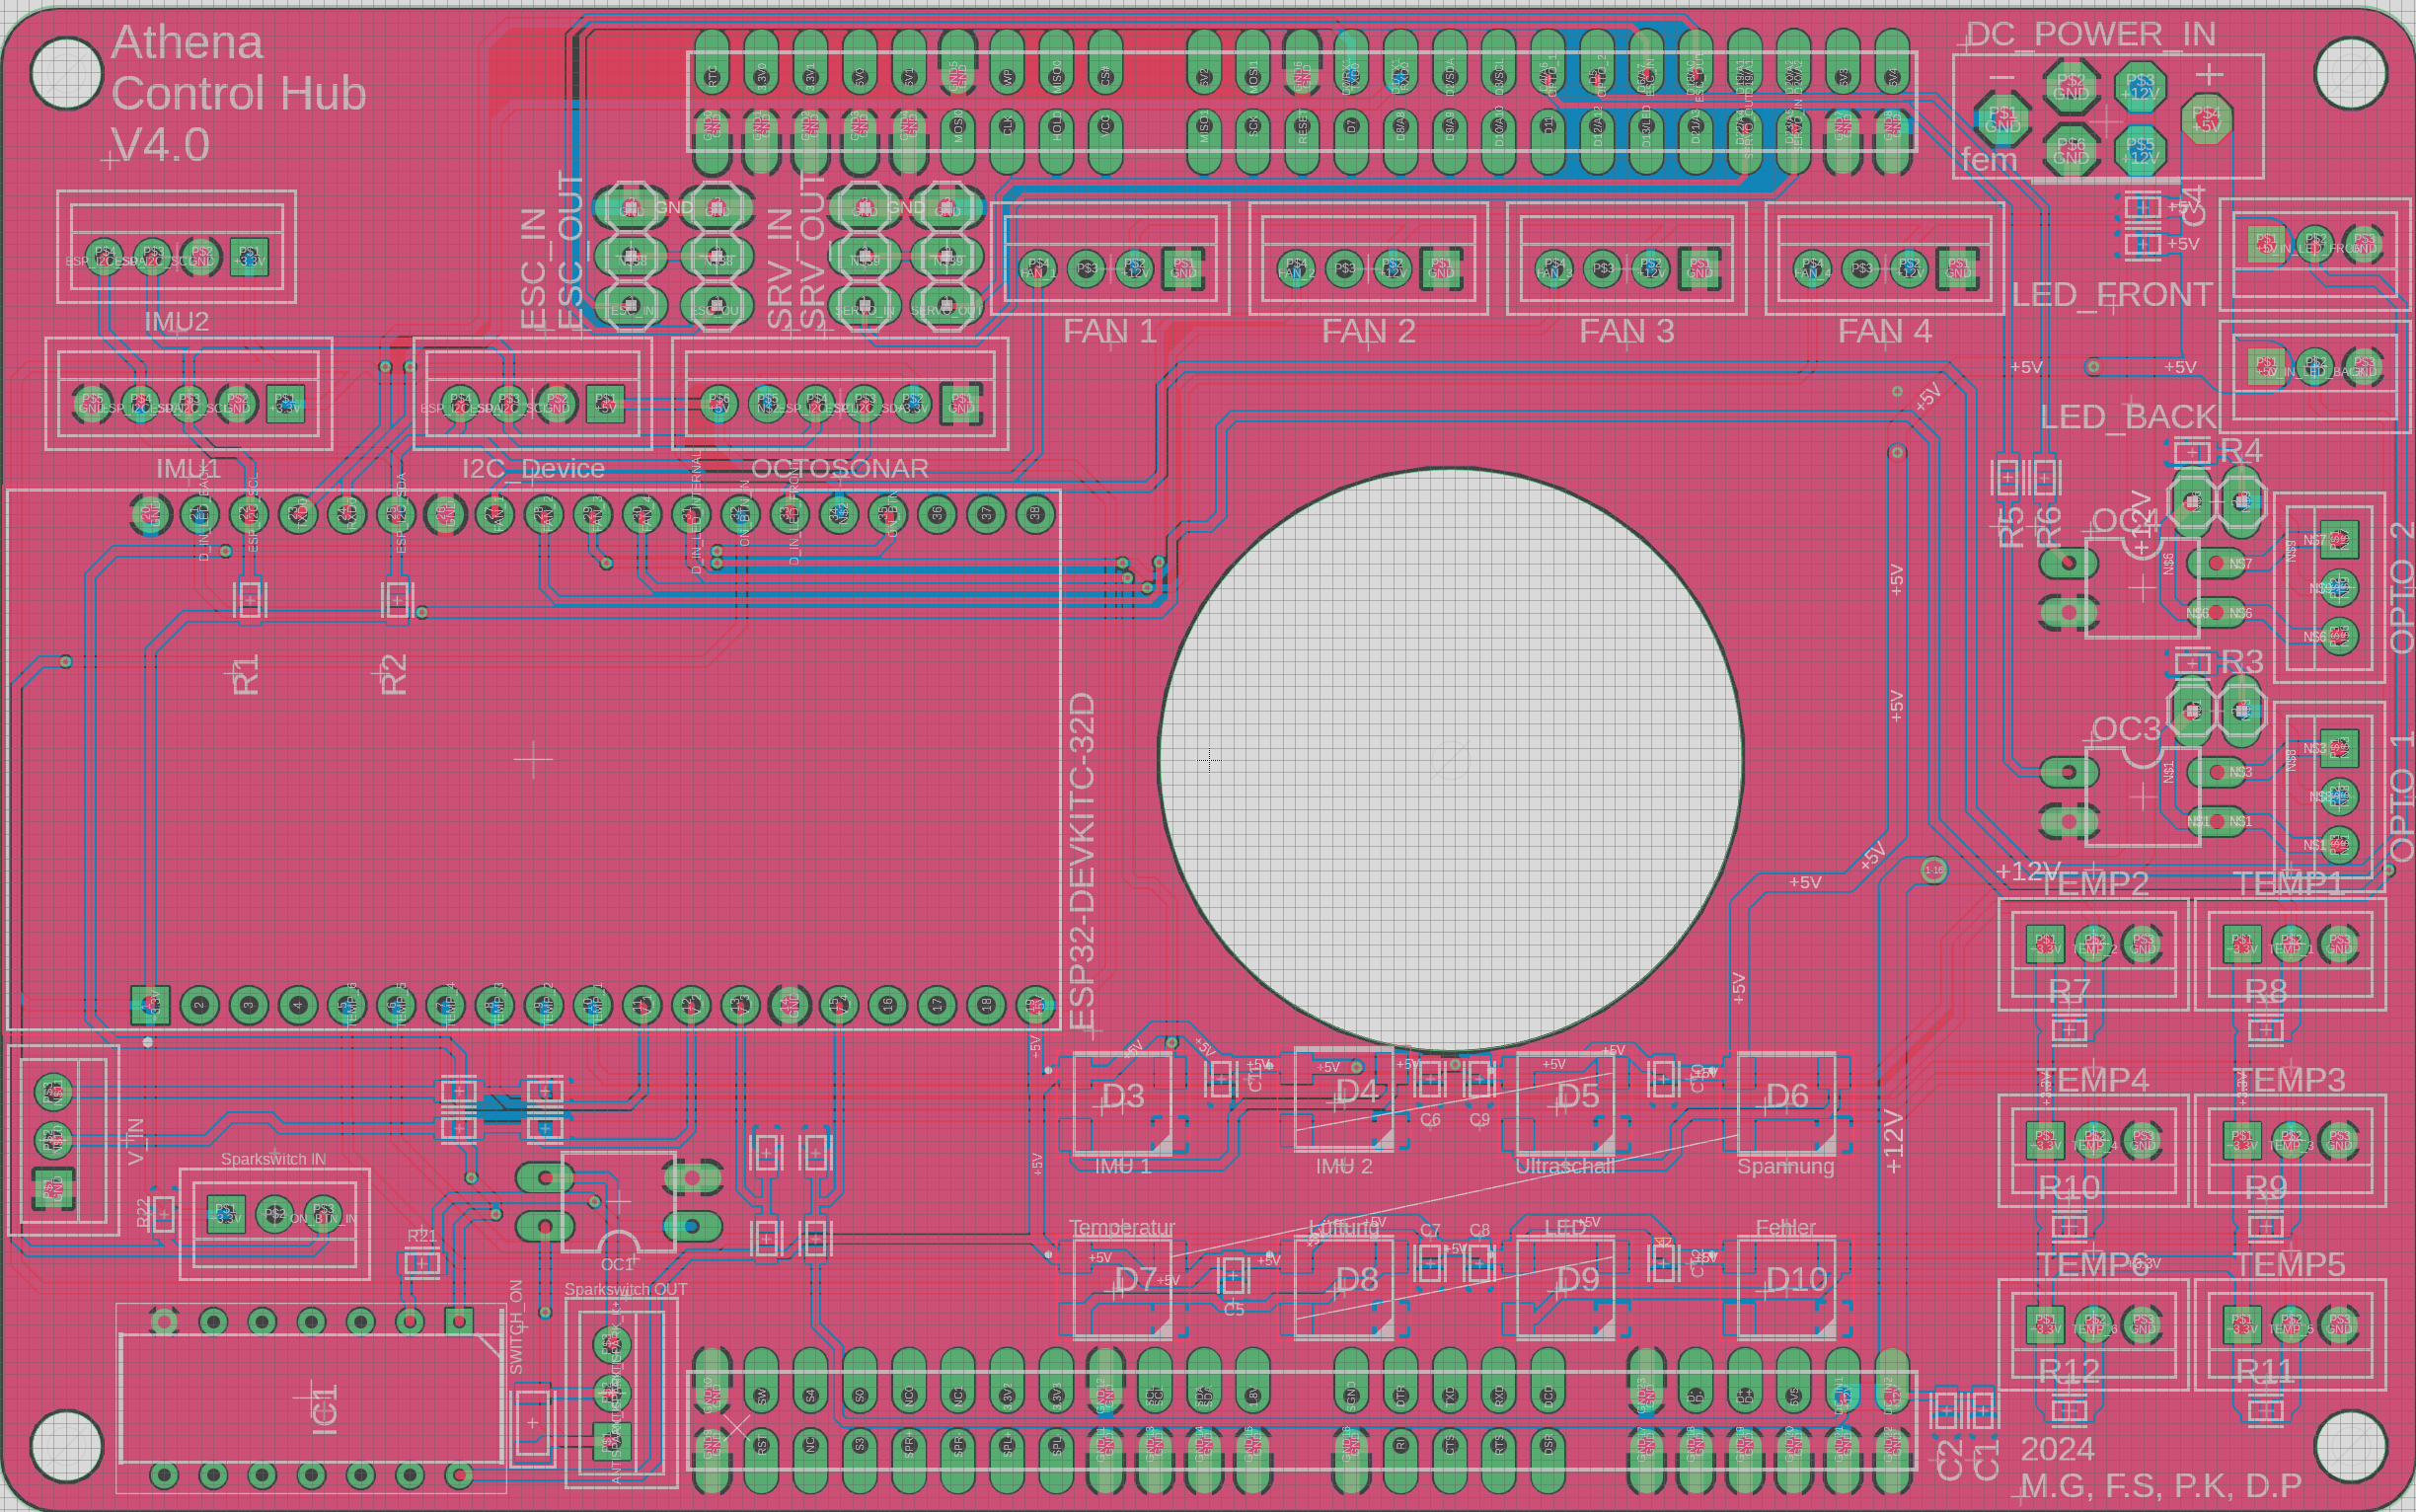
\includegraphics[scale=0.3]{./5_Elektronik/Abbildungen/Platine_1}
			\caption{Vorderseite des Shields}
		\end{figure}
		
		\begin{figure}[H]
			\centering
			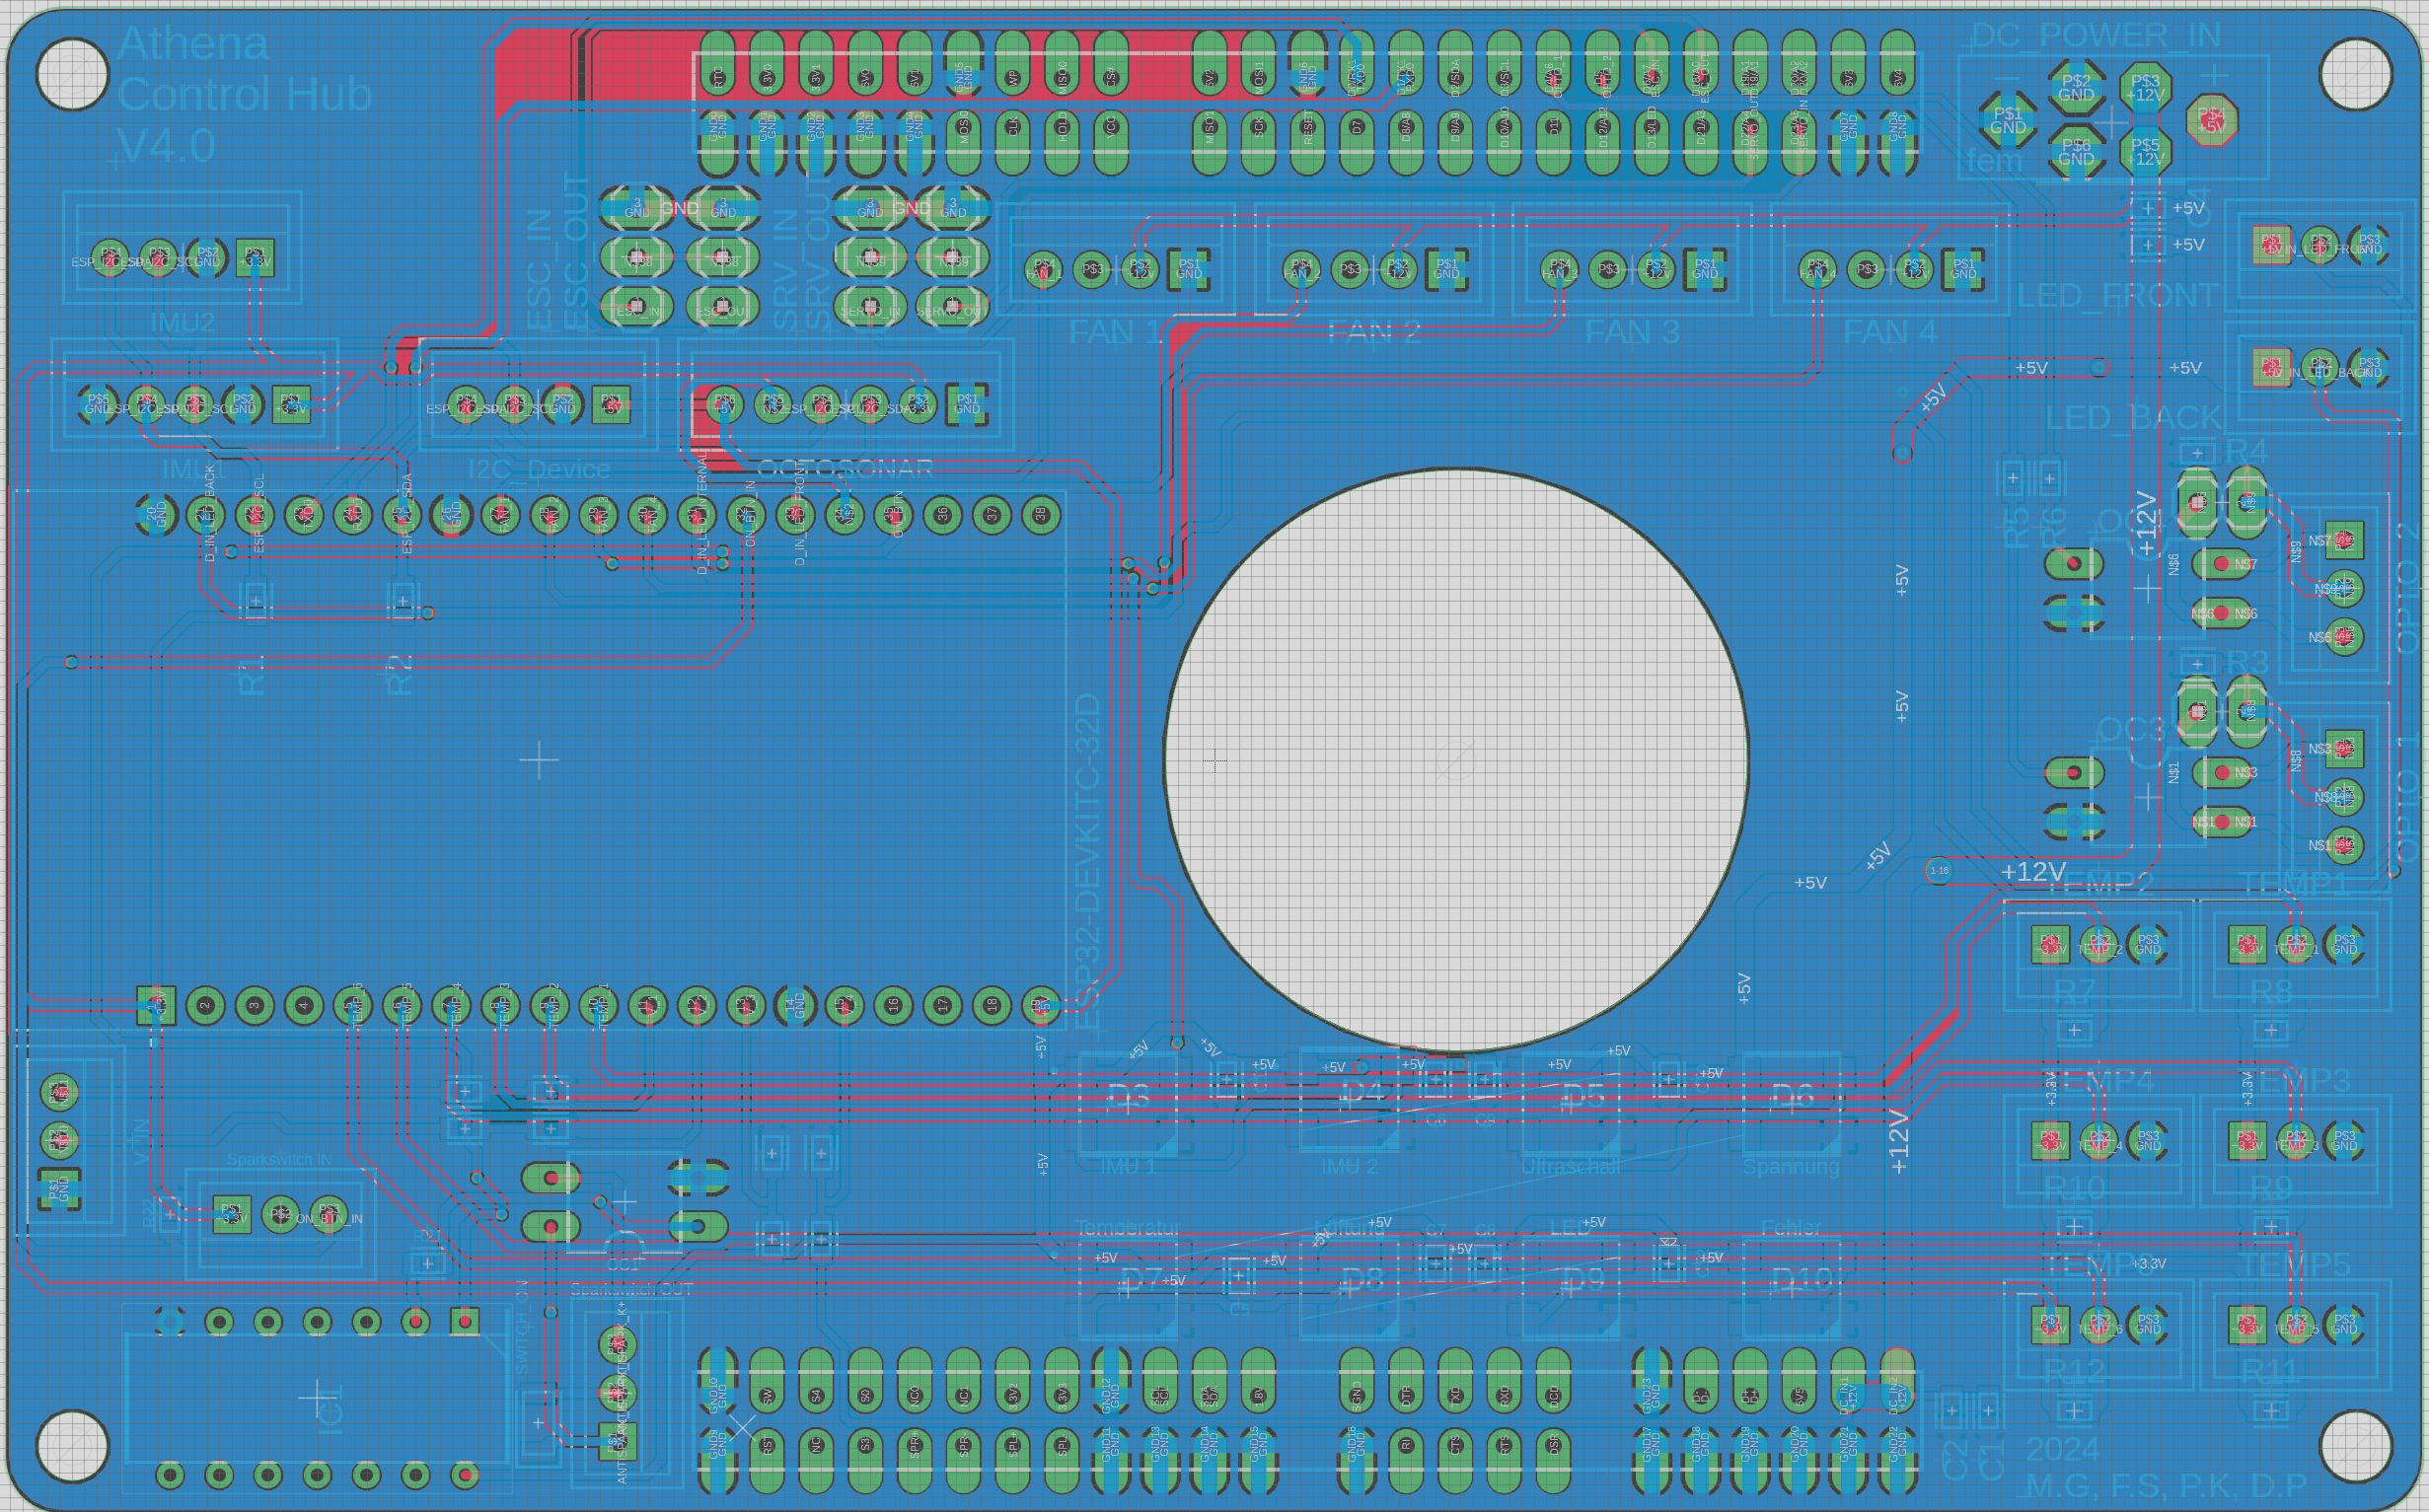
\includegraphics[scale=0.3]{./5_Elektronik/Abbildungen/Platine_2}
			\caption{R�ckseite des Shields}
		\end{figure}
		
		Der Stromlaufplan des Shields ist der Arbeit angeh�ngt.